\section{Overview}

The English word \textit{atom} derives from the Greek
\textgreek{ἄτομος} (átomos, ``uncuttable,'')
itself composed of the etymological ``atoms''
\textgreek{ἀ}- (a-, ``not'')
and
\textgreek{τέμνω } (témnō, ``I cut'').

Stanford Encyclopedia of Philosophy~\cite{sep-atomism-ancient}.
Pythagoras and the monad.
Zeno's paradoxes.
Leucippus and Democritus.
Dalton.
Einstein~\cite{aps_einstein_brownian}.
Rutherford.


Modern understanding of elementary particles.
Dirac.
Fermi's four-fermion interaction.
Feynman and QED.
Electroweak unification.
Strong interaction.
Standard Model of Particle Physics.

\begin{figure}[!h]
    \centering
    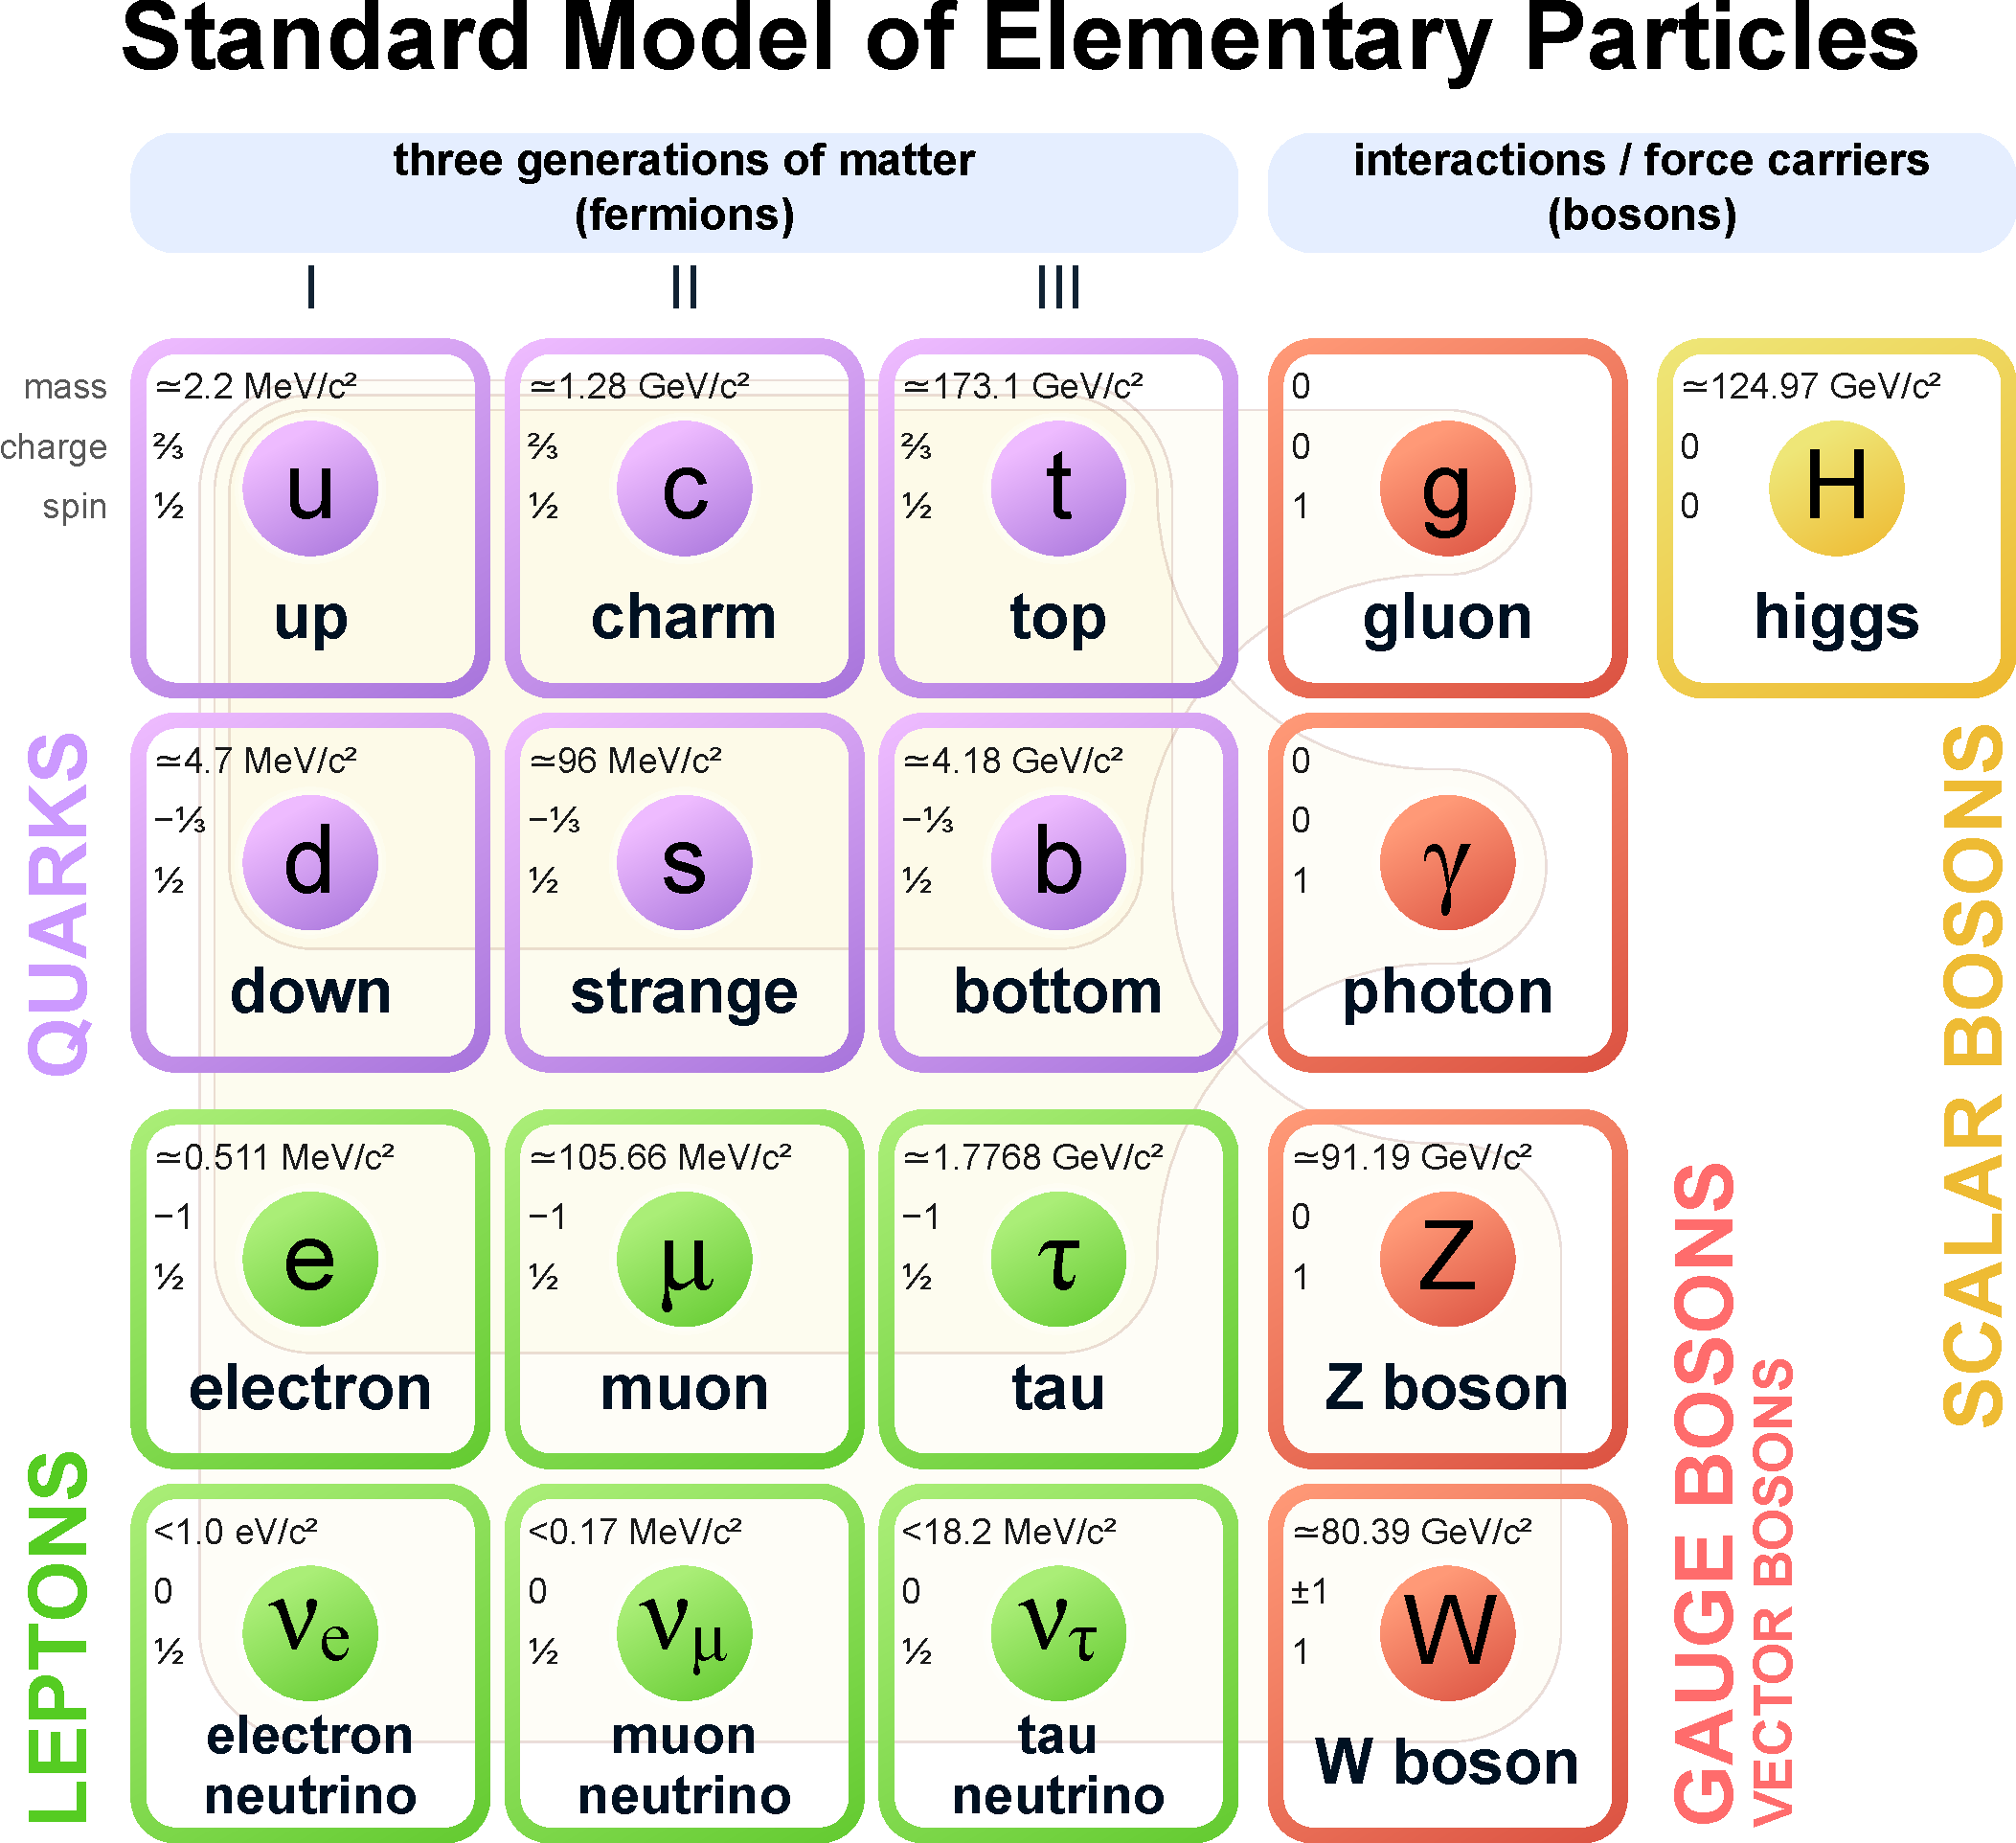
\includegraphics[width=0.6\textwidth]{chap1/Standard_Model_of_Elementary_Particles.pdf}
    \caption{The elementary particles of the Standard Model. Reproduced from
             Wikimedia~\cite{standard_model_wikimedia}.
            }
    \label{fig:Standard_Model_of_Elementary_Particles}
\end{figure}

TODO: make this waaaaaaaaaaaay less colloquial; I copied it from something else I was writing
\subsubsection{Historical uses of particle beams to study nuclear structure}
Around 1910, Rutherford, Geiger, and Marsden used a beam of alpha particles
incident on a gold foil to study atomic structure.
Their results~\cite{Rutherford_1911} suggested that the atom is composed of a
small, dense, positively charged nucleus surrounded by a cloud of electrons.

In the century since, physicists have used other particle beams to study the
substructure of nuclei as well as the nucleons (i.  e.  protons and neutrons)
that compose nuclei.
The culmuniation of decades of such experiments is a theory called quantum
chromodynamics (QCD): the theory that quarks and gluons are the fundamental
building blocks that make up hadrons, a category of composite particles that
includes protons and neutrons.

The Thomas Jefferson National Accelerator Facility (JLab) in Newport News, VA
is home to the Continuous Electron Beam Accelerator Facility (CEBAF).
The CEBAF beam delivers a 12 GeV beam of polarized electrons to four
experimental halls.
Most JLab experiments study the debris produced when the CEBAF electron beam
hits a fixed nuclear target.
By studying this debris, physicists are able to obtain new insights into
nuclear and nucleon structure, exotic configurations of quarks, and other
facets of QCD.

\subsubsection{Scattering in classical physics}
Now what exactly is “quasielastic scattering”?
Elastic scattering is something you might be familiar with from introductory
physics courses.
In Newtonian physics, an elastic collision is one in which kinetic energy is
conserved.
A canonial example is an air hockey puck hitting another puck on a frictionless
plane.
An inelastic collision is one in which kinetic energy is not conserved.
A canonical example is two wads of gum colliding and sticking together in zero
gravity.

\subsubsection{Scattering in nuclear physics}
In nuclear physics, the canonical example of elastic collisions is an electron
colliding with a free proton.
The collision is elastic in the sense that the incoming and outgoing particles
all retain their “identities.”

One of the fun aspects of quantum field theory comes from the intersection of
quantum mechanics and relativity.
Energy and matter are in some sense interchangeable, so some of the energy
contained in colliding particles can be converted into mass.
This is how collisions of proton beams at the LHC create short-lived particles
like the Higgs boson.

At “low” energies, an electron colliding with a nucleus will kick out a proton
or neutron.
Physicists can use this process to study how tightly bound individual nucleons
are in a paritcular nucleus.

At higher energies, some of this $E=mc^2$ energy can be converted into “new”
particles.
Instead of nucleons, particles like pions, kaons, and muons come out of the
collision.
At this energy scale, we start probing sub-nucleon structures instead of
nuclear structures.
Physicsts call these types of interactions “deep inelastic scattering” because
we are using scattering processes to study the “deep” structure of strongly
interacting matter.

Quasielastic scattering is a “low” energy process where the collision looks
like the elastic case of an electron colliding with a free proton.
None of the energy is converted into “new” particles.
The electron transfers momentum to one of a nucleus’s constituent proton,
removing it from its bound state in the nucleus.
This interaction is called “quasielastic” because it looks more like an
electron hitting a free proton than it does a deep inelastic interaction.

